\section{Resultados de los experimentos}

% [1] ¿Cuántos niveles de servidores DNS se recorrieron en las sucesivas consultas hasta obtener la información solicitada?

% [2] ¿Todos los servidores DNS Autoritativos que aparecen en las sucesivas respuestas responden a las consultas realizadas?

% [3] ¿Cuántos nombres de servidores de mail encontraron?, ¿Tienen nombres en el mismo dominio que la universidad?

% [4] ¿Cuántas direcciones IP distintas hay? ¿Estas direcciones IP corresponden a dispositivos que están prendidos? (Hint: probar con ping si responden)

% [5] ¿Coinciden las IPs de los servidores de correo con las IPs de los servidores Web?

\subsection{Departamento de Computación - FCEyN UBA}
% www.dc.uba.ar

% Comentario... si hacemos el experimento con la UBA (www.uba.ar) no conseguimos ningún MX. esto puede que se el mismo caso para algunas de las tras universidades que probamos, tal vez habia que pegarle a alguna facultad o unidad academica específica dentro de cada una (...)

% [1]
Se recorrieron 3 niveles para todos los root servers con los que se comenzó.
Los primeros dos variaron en las distintas repeticiones del experimento pero el final fue siempre el mismo: \textsc{ns1.uba.ar-157.92.1.1}.

\begin{center}
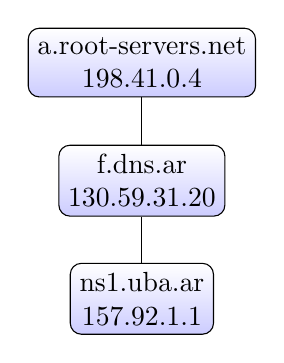
\begin{tikzpicture}[sibling distance=10em,
  every node/.style = {shape=rectangle, rounded corners,
    draw, align=center,
    top color=white, bottom color=blue!20}]]
  \node {a.root-servers.net\\198.41.0.4}
    child { node {f.dns.ar\\130.59.31.20 }
      child { node {ns1.uba.ar\\157.92.1.1} } };
\end{tikzpicture}
\captionof{figure}{Árbol de consultas DNS para www.dc.uba.ar comenzando con a.root-servers.net.}
\label{fig:dcubaar_a_tree} 
\end{center}

% [2]
Todos respondieron a las consultas realizadas.

% [3]
Encontramos dos nombres de servidores de mail: \textsc{mta0.fcen.uba.ar} y \textsc{mta1.fcen.uba.ar}, los mismos coinciden con el dominio del departamento: \textsc{uba.ar}.

% [5]
No coinciden las \textsc{IPs} de los servidores de correo con la \textsc{IPs} del servidor Web. Todas las direcciones corresponden a la misma zona geográfica de Buenos Aires.
% www.dc.uba.ar    157.92.27.128
% mta0.fcen.uba.ar 157.92.32.130
% mta1.fcen.uba.ar 157.92.32.131


\subsection{Universidad Nacional Arturo Jauretche}
% www.unaj.edu.ar

% [1]
En un caso se recorrieron tres niveles \textsc{DNS} hasta obtener la respuesta (similar a \ref{fig:dcubaar_a_tree}). En los otros dos se llegó a recorrer cuatro. En \ref{fig:unajedu_c_tree} se muestra el árbol producido por comenzar con el root server c.

\begin{center}
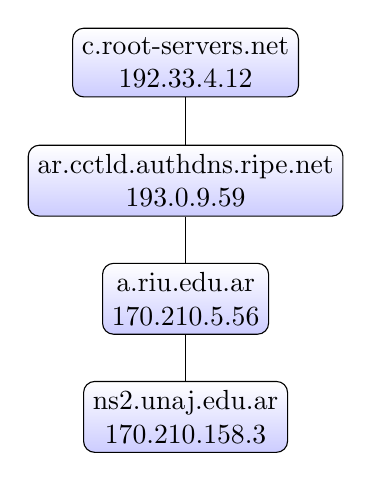
\begin{tikzpicture}[sibling distance=10em,
  every node/.style = {shape=rectangle, rounded corners,
    draw, align=center,
    top color=white, bottom color=blue!20}]]
  \node {c.root-servers.net\\192.33.4.12}
    child { node {ar.cctld.authdns.ripe.net\\193.0.9.59 }
      child { node {a.riu.edu.ar\\170.210.5.56}
        child { node {ns2.unaj.edu.ar\\170.210.158.3} } } };
\end{tikzpicture}
\captionof{figure}{Árbol de consultas DNS para www.unaj.edu.ar comenzando con c.root-servers.net.}
\label{fig:unajedu_c_tree} 
\end{center}

% [2]
Todos respondieron a las consultas realizadas.

% [3]
Encontramos un nombre de servidor de mail: \textsc{mail.unaj.edu.ar}. Coincide con el dominio de la universidad.

% [5]
No coinciden las \textsc{IPs} de los servidores de correo con la \textsc{IPs} del servidor Web. Ambas pertenecen a la Red de Interconexión Universitaria, en Argentina.
% www.unaj.edu.ar 170.210.44.19
% mail.unaj.edu.ar 170.210.44.22

\newpage

\subsection{Universidad Nacional de Formosa}
% www.unf.edu.ar

% [1]
En dos casos cuatro niveles de \textsc{DNS} fue necesario recorrer para obtener la respuesta, en otro caso fueron necesarios solo tres. En \ref{fig:unfedu_b_tree} se muestra el árbol producido por comenzar con el root server b.

\begin{center}
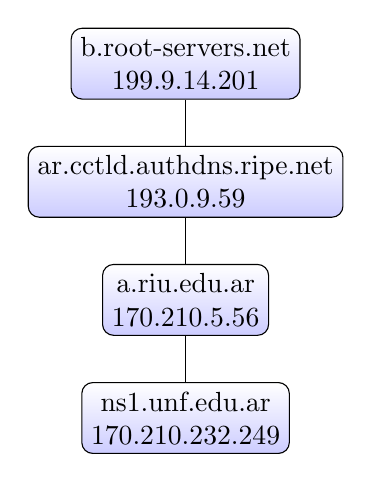
\begin{tikzpicture}[sibling distance=10em,
  every node/.style = {shape=rectangle, rounded corners,
    draw, align=center,
    top color=white, bottom color=blue!20}]]
  \node {b.root-servers.net\\199.9.14.201}
    child { node {ar.cctld.authdns.ripe.net\\193.0.9.59 }
      child { node {a.riu.edu.ar\\170.210.5.56}
        child { node {ns1.unf.edu.ar\\170.210.232.249} } } };
\end{tikzpicture}
\captionof{figure}{Árbol de consultas DNS para www.unf.edu.ar comenzando con b.root-servers.net.}
\label{fig:unfedu_b_tree} 
\end{center}

% [2]
Todos respondieron a las consultas realizadas.

% [3]
Coincide el dominio de la universidad con el nombre del unico servidor de mail encontrado: \textsc{mail.unf.edu.ar}.

% [5]
La \textsc{IP} del servidor de correo y la \textsc{IP} del servidor web coinciden: \textsc{170.210.232.249}. Ambas pertenecen a la Red de Interconexión Universitaria, en Argentina.
% www.unf.edu.ar 170.210.232.249
% mail.unf.edu.ar 170.210.232.249

\subsection{Universidad de Tübingen}
% www.uni-tuebingen.de

% [1]
En todas las iteraciones del experimento fueron necesarios 3 niveles de \textsc{DNS} para alcanzar la respuesta. El árbol de consultas generado comenzando desde el root server a se puede ver en \ref{fig:tubingen_a_tree}.

\begin{center}
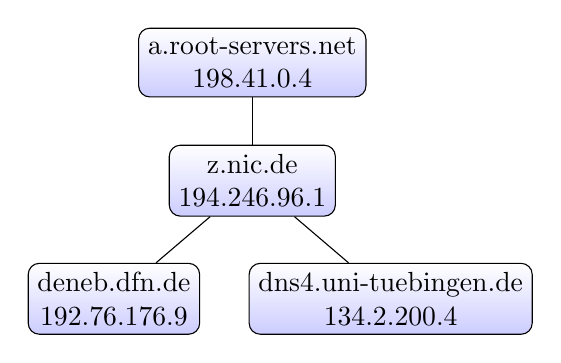
\begin{tikzpicture}[sibling distance=10em,
  every node/.style = {shape=rectangle, rounded corners,
    draw, align=center,
    top color=white, bottom color=blue!20}]]
  \node {a.root-servers.net\\198.41.0.4}
    child { node {z.nic.de\\194.246.96.1 }
      child { node {deneb.dfn.de\\192.76.176.9} }
      child { node {dns4.uni-tuebingen.de\\134.2.200.4} } };
\end{tikzpicture}
\captionof{figure}{Árbol de consultas DNS para www.uni-tuebingen.de comenzando con a.root-servers.net.}
\label{fig:tubingen_a_tree} 
\end{center}

% [2]
Uno de los cuatro servidores consultados nunca respondió. Este es \textsc{deneb.dfn.de} (\textsc{192.76.176.9}). Se obtuvo respuesta al hacer ping con este servidor por lo que no está apagado, así que se debe a otro motivo que no responda las consultas \textsc{DNS} que se le hace.

% [3]
Cinco fueron los nombres de servidores de mails encontrados, de los cuales dos coinciden con el dominio de la universidad (\textsc{mx05.uni-tuebingen.de} y \textsc{mx06.uni-tuebingen.de}) y los otros tres pertenecen a la Red de Investigación Alemana (German Research Network (DFN)) y son: \textsc{a1541.mx.srv.dfn.de}, \textsc{b1541.mx.srv.dfn.de} y \textsc{c1541.mx.srv.dfn.de}.

% [5]
% www.uni-tuebingen.de 134.2.5.1
% a1541.mx.srv.dfn.de 194.95.232.90
% b1541.mx.srv.dfn.de 194.95.234.90
% c1541.mx.srv.dfn.de 194.95.238.90
% mx05.uni-tuebingen.de 134.2.5.215
% mx06.uni-tuebingen.de 134.2.5.216
No coinciden las IPs de los servidores de correo con la IPs del servidor Web.

El servidor web y los servidores de correo \textsc{mx05.uni-tuebingen.de} y \textsc{mx06.uni-tuebingen.de} pertenecen a la zona de la ciudad de Landkreis Tuebingen en la región de Baden-Württemberg en Alemania.

Los servidores \textsc{a1541.mx.srv.dfn.de}, \textsc{b1541.mx.srv.dfn.de} y \textsc{c1541.mx.srv.dfn.de} con IPs \textsc{194.95.232.90}, \textsc{194.95.234.90} y \textsc{194.95.238.90} respectivamente, están localizados en Kassel, una ciudad en Hessel, Alemania.

En \ref{fig:tubingen_map} mostramos la ubicación geográfica de los servidores web y correo de Tübingen y los de correo de la German Research Network.

\begin{figure}[H]
  \centering
  \includegraphics[width=1\textwidth]{imagenes/tubingen.png}
  \caption{Distancia geográfica entre la Universidad de Tübingen y la German Research Network}
  \label{fig:tubingen_map}
\end{figure}